\documentclass[titlepage,a4paper]{article}

\usepackage{cmap}
\usepackage[T1]{fontenc}
\usepackage[utf8]{inputenc}
\usepackage[swedish]{babel}
\usepackage{graphicx}
\usepackage{hyperref} 	 
	
\title{Projekt 2, EIT060 Datasäkerhet}

\author{Emil Persson, dat11epe\\
Valdemar Roxling, dat11vro}

\begin{document}

\maketitle

\tableofcontents

\newpage

\section{Introduktion}
 Hej
\section{System \& Design}

\begin{figure}[!h]
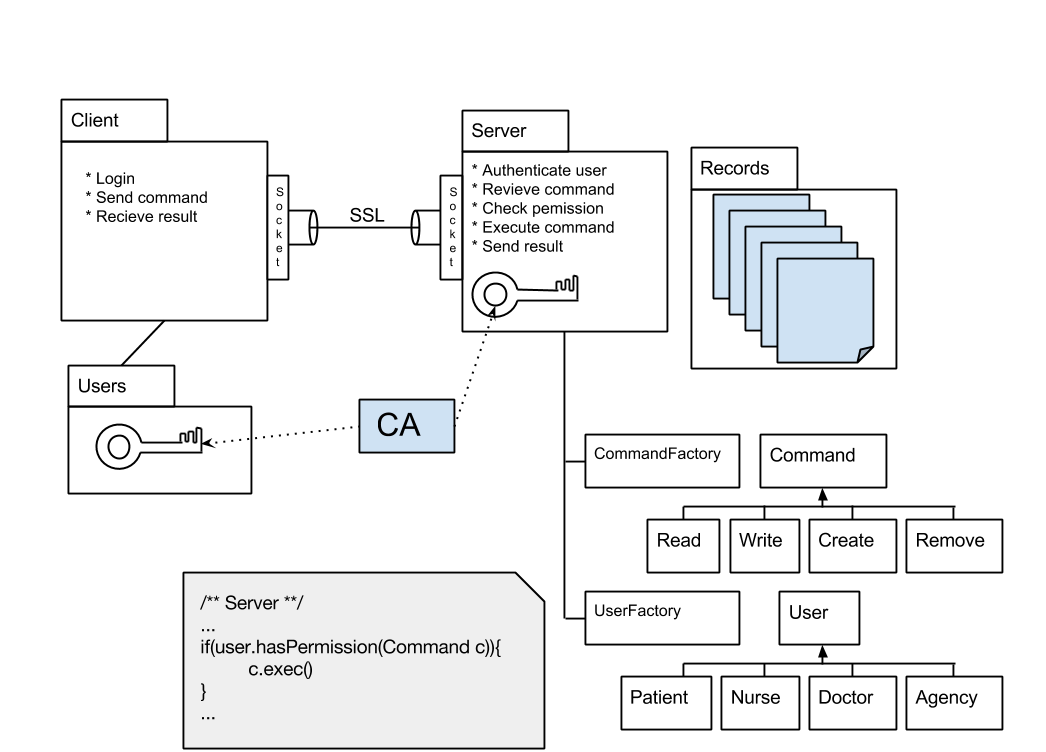
\includegraphics[width=\textwidth]{Design.png}
\caption{Systemdesign}
\label{design}
\end{figure}
 lite system och design
\section{Säkerhetsanalys  \& Attacker}
\begin{enumerate}
\item Man in the middle

\item Spoofing
\end{enumerate}



\section{Beskrivning av SSL}
nästan slut
\end{document}
